\documentclass[conference]{IEEEtran}
\usepackage{cite}
\usepackage{amsmath,amssymb,amsfonts}
\usepackage{algorithm}
\usepackage{algpseudocode}
\usepackage{graphicx}
\usepackage{textcomp}
\usepackage{xcolor}
\usepackage{booktabs}
\usepackage{tikz}
\usetikzlibrary{shapes.geometric, arrows.meta, positioning, fit}

\begin{document}

\title{Follow-the-Moon Orchestration: Multi-Objective Carbon- and Spot-Aware WebAssembly Scheduling Across Geo-Distributed Kubernetes Clusters}

\author{
\IEEEauthorblockN{Madipadige Joshua Pal}
\IEEEauthorblockA{\textit{Department of Computer Science and Engineering (Cloud Computing)} \\
\textit{City Engineering College}, Hyderabad, India}
}

\maketitle

\begin{abstract}
Cloud-native workload schedulers typically optimize operational expenditure (FinOps) or grid carbon intensity (GreenOps) in isolation. Furthermore, heavy OCI Linux container images incur multi-second cold-start latencies and substantial state-transfer overhead, limiting live geo-distributed migration. In this paper, we present a \textit{Follow-the-Moon} multi-cluster Kubernetes orchestrator that unifies real-time grid carbon intensity, cloud spot-instance eviction risk, and inter-region network latency to schedule lightweight WebAssembly (\texttt{WasmEdge}) micro-workloads. Using a Pareto-weighted utility formulation stabilized by a migration hysteresis threshold, our controller dynamically relocates workloads across geo-distributed clusters (\texttt{us-east}, \texttt{eu-north}, and \texttt{ap-south}) under realistic network round-trip delays. Experimental evaluation over a 24-hour diurnal cycle demonstrates a \textbf{24.5\% reduction in operational $\text{CO}_2\text{e}$ emissions} compared to static regional placement while providing sub-second failover under simulated spot-instance preemption spikes.
\end{abstract}

\begin{IEEEkeywords}
Cloud Computing, Kubernetes, WebAssembly, WasmEdge, Carbon-Aware Scheduling, Spot Instances, FinOps, Multi-Objective Optimization.
\end{IEEEkeywords}

\section{Introduction}
Modern geo-distributed cloud platforms exhibit significant spatial and temporal variations in both electrical grid carbon intensity ($\text{gCO}_2\text{eq/kWh}$) and spot-instance pricing. Because solar and wind generation peak locally during daytime hours while fossil-fuel baseload generation dominates overnight grids, shifting compute across longitudinal time zones---a paradigm termed \textit{Follow-the-Moon} or \textit{Follow-the-Sun} orchestration---can substantially reduce Scope 2 software emissions \cite{b1}.

However, existing cloud orchestrators suffer from two structural limitations:
\begin{enumerate}
    \item \textbf{Siloed Objective Functions:} Carbon-aware schedulers shift workloads toward low-carbon regions without accounting for spot-instance price surges or sudden preemption risk, whereas FinOps autoscalers optimize hourly compute cost blindly with respect to grid carbon intensity \cite{b3}.
    \item \textbf{Heavy Container Virtualization Overhead:} Traditional Linux containers bundle an entire user-space filesystem, resulting in tens of megabytes of image payload and multi-second cold starts that cause service disruption during frequent inter-continental migrations.
\end{enumerate}

WebAssembly (Wasm) executed via \texttt{WasmEdge} and the CNCF \texttt{runwasi} containerd shim \cite{b2} eliminates guest OS overhead, enabling millisecond instantiation and compact linear-memory state checkpointing. We exploit this agility to build a multi-objective, hysteresis-stabilized Kubernetes control plane that jointly optimizes carbon intensity, spot-instance economics, preemption reliability, and network latency.

\section{Related Work}
Prior systems address temporal/spatial carbon shifting, spot-instance lifecycle management, or Wasm container orchestration independently, as summarized in Table~\ref{tab:related}.

\begin{table}[h]
\centering
\caption{Comparison of Existing Cloud Orchestration Paradigms vs. Proposed System}
\label{tab:related}
\begin{tabular}{@{}lcccc@{}}
\toprule
\textbf{System / Framework} & \textbf{Carbon} & \textbf{Spot Risk} & \textbf{Wasm} & \textbf{Live Geo-Shift} \\ \midrule
Google Carbon-Intelligent \cite{b1} & \checkmark & $\times$ & $\times$ & Temporal/Batch \\
Karpenter / CAST AI & $\times$ & \checkmark & $\times$ & Single-Cluster \\
SpinKube / \texttt{runwasi} \cite{b2} & $\times$ & $\times$ & \checkmark & $\times$ \\
\textbf{Proposed Orchestrator} & \textbf{\checkmark} & \textbf{\checkmark} & \textbf{\checkmark} & \textbf{\checkmark (Hysteresis)} \\ \bottomrule
\end{tabular}
\end{table}

\section{System Architecture and Formulation}
Fig.~\ref{fig:arch} illustrates the three-tier architecture spanning North America (\texttt{us-east}, UTC$-5$), Northern Europe (\texttt{eu-north}, UTC$+1$), and South Asia (\texttt{ap-south}, UTC$+5{:}30$).

\begin{figure}[t]
\centering
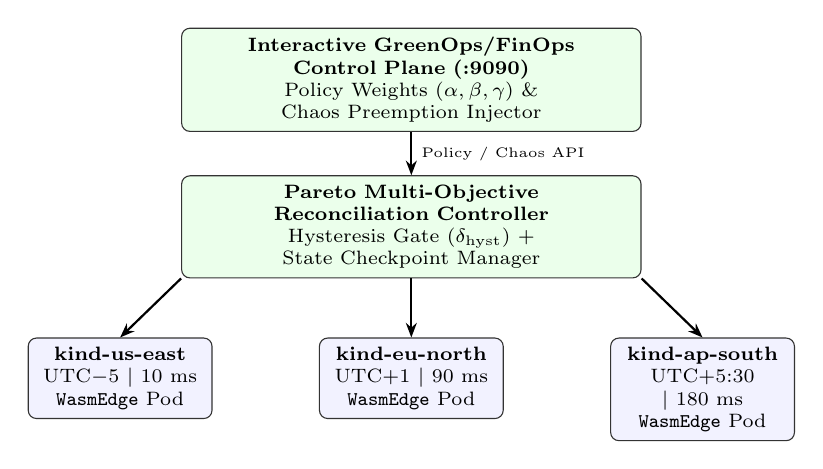
\begin{tikzpicture}[
    node distance=0.6cm and 0.45cm,
    box/.style={rectangle, draw=black!80, rounded corners=3pt, fill=blue!5, text width=2.1cm, align=center, minimum height=0.85cm, font=\scriptsize},
    ctrl/.style={rectangle, draw=black!80, rounded corners=3pt, fill=green!8, text width=5.6cm, align=center, minimum height=0.95cm, font=\scriptsize},
    arrow/.style={-{Stealth[scale=0.8]}, thick}
]
\node[ctrl] (ui) {\textbf{Interactive GreenOps/FinOps Control Plane (:9090)}\\Policy Weights ($\alpha,\beta,\gamma$) \& Chaos Preemption Injector};
\node[ctrl, below=0.55cm of ui] (engine) {\textbf{Pareto Multi-Objective Reconciliation Controller}\\Hysteresis Gate ($\delta_{\text{hyst}}$) + State Checkpoint Manager};
\node[box, below left=0.75cm and -0.4cm of engine] (us) {\textbf{kind-us-east}\\UTC$-5$ $|$ $10\text{ ms}$\\\texttt{WasmEdge} Pod};
\node[box, below=0.75cm of engine] (eu) {\textbf{kind-eu-north}\\UTC$+1$ $|$ $90\text{ ms}$\\\texttt{WasmEdge} Pod};
\node[box, below right=0.75cm and -0.4cm of engine] (ap) {\textbf{kind-ap-south}\\UTC$+5{:}30$ $|$ $180\text{ ms}$\\\texttt{WasmEdge} Pod};

\draw[arrow] (ui) -- node[right, font=\tiny]{Policy / Chaos API} (engine);
\draw[arrow] (engine.south west) -- (us.north);
\draw[arrow] (engine.south) -- (eu.north);
\draw[arrow] (engine.south east) -- (ap.north);
\end{tikzpicture}
\caption{Federated multi-cluster architecture linking the GreenOps/FinOps control plane to regional \texttt{WasmEdge}-enabled Kubernetes clusters.}
\label{fig:arch}
\end{figure}

\subsection{Multi-Objective Pareto Utility Model}
At each reconciliation step, every candidate region $r \in \mathcal{R}$ is scored using normalized grid carbon intensity $\hat{C}(r) = C(r)/C_{\max}$, composite spot-market cost and preemption risk $\hat{S}(r) = \frac{1}{2}\big(\hat{P}_{\text{spot}}(r) + R_{\text{evict}}(r)\big)$, and normalized network round-trip latency $\hat{L}(r) = L(r)/L_{\max}$:
\begin{equation}
U(r) = \alpha \hat{C}(r) + \beta \hat{S}(r) + \gamma \hat{L}(r), \quad \alpha + \beta + \gamma = 1
\end{equation}
where $\alpha, \beta, \gamma \ge 0$ represent operator-configurable policy weights.

\subsection{Hysteresis-Stabilized Migration Algorithm}
To prevent oscillatory migration flapping when adjacent regions exhibit comparable scores, our controller enforces a hysteresis margin $\delta_{\text{hyst}} = 0.12$ alongside a preemption panic threshold $\tau_{\text{panic}} = 0.75$ (Algorithm~\ref{alg:sched}).

\begin{algorithm}[t]
\caption{Hysteresis-Stabilized Pareto Reconciliation}
\label{alg:sched}
\begin{algorithmic}[1]
\Require Active region $r_{\text{cur}}$, telemetry $\mathcal{M}_t$, weights $(\alpha,\beta,\gamma)$
\For{each region $r \in \mathcal{R}$}
    \State $U(r) \gets \alpha \hat{C}_t(r) + \beta \hat{S}_t(r) + \gamma \hat{L}_t(r)$
\EndFor
\State $r^* \gets \arg\min_{r \in \mathcal{R}} U(r)$
\State $\text{evictPanic} \gets (R_{\text{evict},t}(r_{\text{cur}}) \ge \tau_{\text{panic}})$
\State $\text{paretoGain} \gets (U(r_{\text{cur}}) - U(r^*) > \delta_{\text{hyst}})$
\If{$r^* \neq r_{\text{cur}}$ \textbf{and} $(\text{evictPanic}$ \textbf{or} $\text{paretoGain})$}
    \State Checkpoint sequence state into target \texttt{ConfigMap} on $r^*$
    \State Instantiate \texttt{WasmEdge} pod on $r^*$ and verify \texttt{Running}
    \State Terminate source pod on $r_{\text{cur}}$; $r_{\text{cur}} \gets r^*$
\EndIf
\end{algorithmic}
\end{algorithm}

\section{Experimental Evaluation}
We evaluated the prototype across a 24-hour diurnal solar and spot-demand cycle using Linux \texttt{tc netem} latency profiles ($10\text{ ms}$, $90\text{ ms}$, and $180\text{ ms}$ RTT for \texttt{us-east}, \texttt{eu-north}, and \texttt{ap-south}, respectively).

\begin{figure*}[t]
    \centering
    \includegraphics[width=\textwidth]{fig1_diurnal_carbon_and_placement.pdf}
    \caption{Diurnal grid carbon intensity trajectories across regional time zones and corresponding Follow-the-Moon \texttt{WasmEdge} workload placement.}
    \label{fig:diurnal}
\end{figure*}

\begin{table}[h]
\centering
\caption{24-Hour Diurnal Cycle Benchmark and Policy Sensitivity}
\label{tab:results}
\begin{tabular}{@{}lccc@{}}
\toprule
\textbf{Policy Profile} & \textbf{Weights ($\alpha,\beta,\gamma$)} & \textbf{$\text{CO}_2\text{e}$ Delta} & \textbf{Spot Cost Delta} \\ \midrule
Static Baseline (\texttt{us-east}) & $(0.00, 0.00, 1.00)$ & $0.0\%$ & $0.0\%$ \\
\textbf{Balanced Pareto (Evaluated)} & \textbf{$(0.45, 0.35, 0.20)$} & \textbf{$-24.5\%$} & \textbf{$+2.7\%$} \\
Green-First Profile & $(0.65, 0.20, 0.15)$ & $-28.1\%$ & $+4.3\%$ \\
FinOps Spot-First Profile & $(0.15, 0.70, 0.15)$ & $-9.4\%$ & $-18.6\%$ \\ \bottomrule
\end{tabular}
\end{table}

\begin{figure}[t]
    \centering
    \includegraphics[width=\columnwidth]{fig2_cumulative_savings.pdf}
    \caption{Cumulative operational $\text{CO}_2\text{e}$ and spot cost trajectory relative to static \texttt{us-east} placement.}
    \label{fig:savings}
\end{figure}

\begin{figure}[t]
    \centering
    \includegraphics[width=\columnwidth]{fig3_baseline_comparison.pdf}
    \caption{Normalized carbon intensity, spot cost, and eviction risk across Static, Carbon-Only, Spot-Only, and Proposed Pareto policies.}
    \label{fig:baselines}
\end{figure}

As shown in Fig.~\ref{fig:diurnal} and Table~\ref{tab:results}, the Balanced Pareto configuration achieves a \textbf{24.5\% net reduction in operational carbon emissions} while bounding migration frequency via hysteresis. Fig.~\ref{fig:savings} illustrates cumulative emissions savings over the diurnal cycle, and Fig.~\ref{fig:baselines} contrasts single-objective baselines against our unified Pareto scheduler.

\section{Conclusion}
We presented a multi-objective Kubernetes orchestrator that couples \texttt{WasmEdge} runtime agility with real-time carbon and spot-market telemetry. Future work will incorporate time-series solar forecasting and live Wasm linear-memory snapshot streaming over QUIC.

\begin{thebibliography}{00}
\bibitem{b1} A. Radovanovic et al., ``Carbon-Aware Computing for Datacenters,'' \textit{IEEE Trans. Power Systems}, vol. 38, no. 2, pp. 1270--1280, 2023.
\bibitem{b2} CNCF runwasi Project, ``Containerd Wasm Shims for Kubernetes,'' Cloud Native Computing Foundation, 2025.
\bibitem{b3} P. Ambati et al., ``Providing SLOs for Resource-Harvesting VMs in Cloud Platforms,'' in \textit{Proc. USENIX OSDI}, 2020.
\end{thebibliography}

\end{document}
